\documentclass{article}
\usepackage{graphicx}
\title{IITB AI accelerator architecture}
\author{Madhav P. Desai \\ Department of Electrical Engineering, IIT Bombay \\ email: madhav@ee.iitb.ac.in}
\begin{document}
\maketitle


\section{Overview}

We describe the architectural base of the AI accelerator algorithm description.
The algorithm itself will be described by 
\begin{itemize}
\item C code.
\item {\bf Aa} code.
\item Hierarchical system description code ({\bf hsys} code).
\end{itemize}

The system being described is hierarchical and the
hiearchy can be visualized as shown in Figure \ref{fig:hierarchy}.
\begin{figure}
\centering
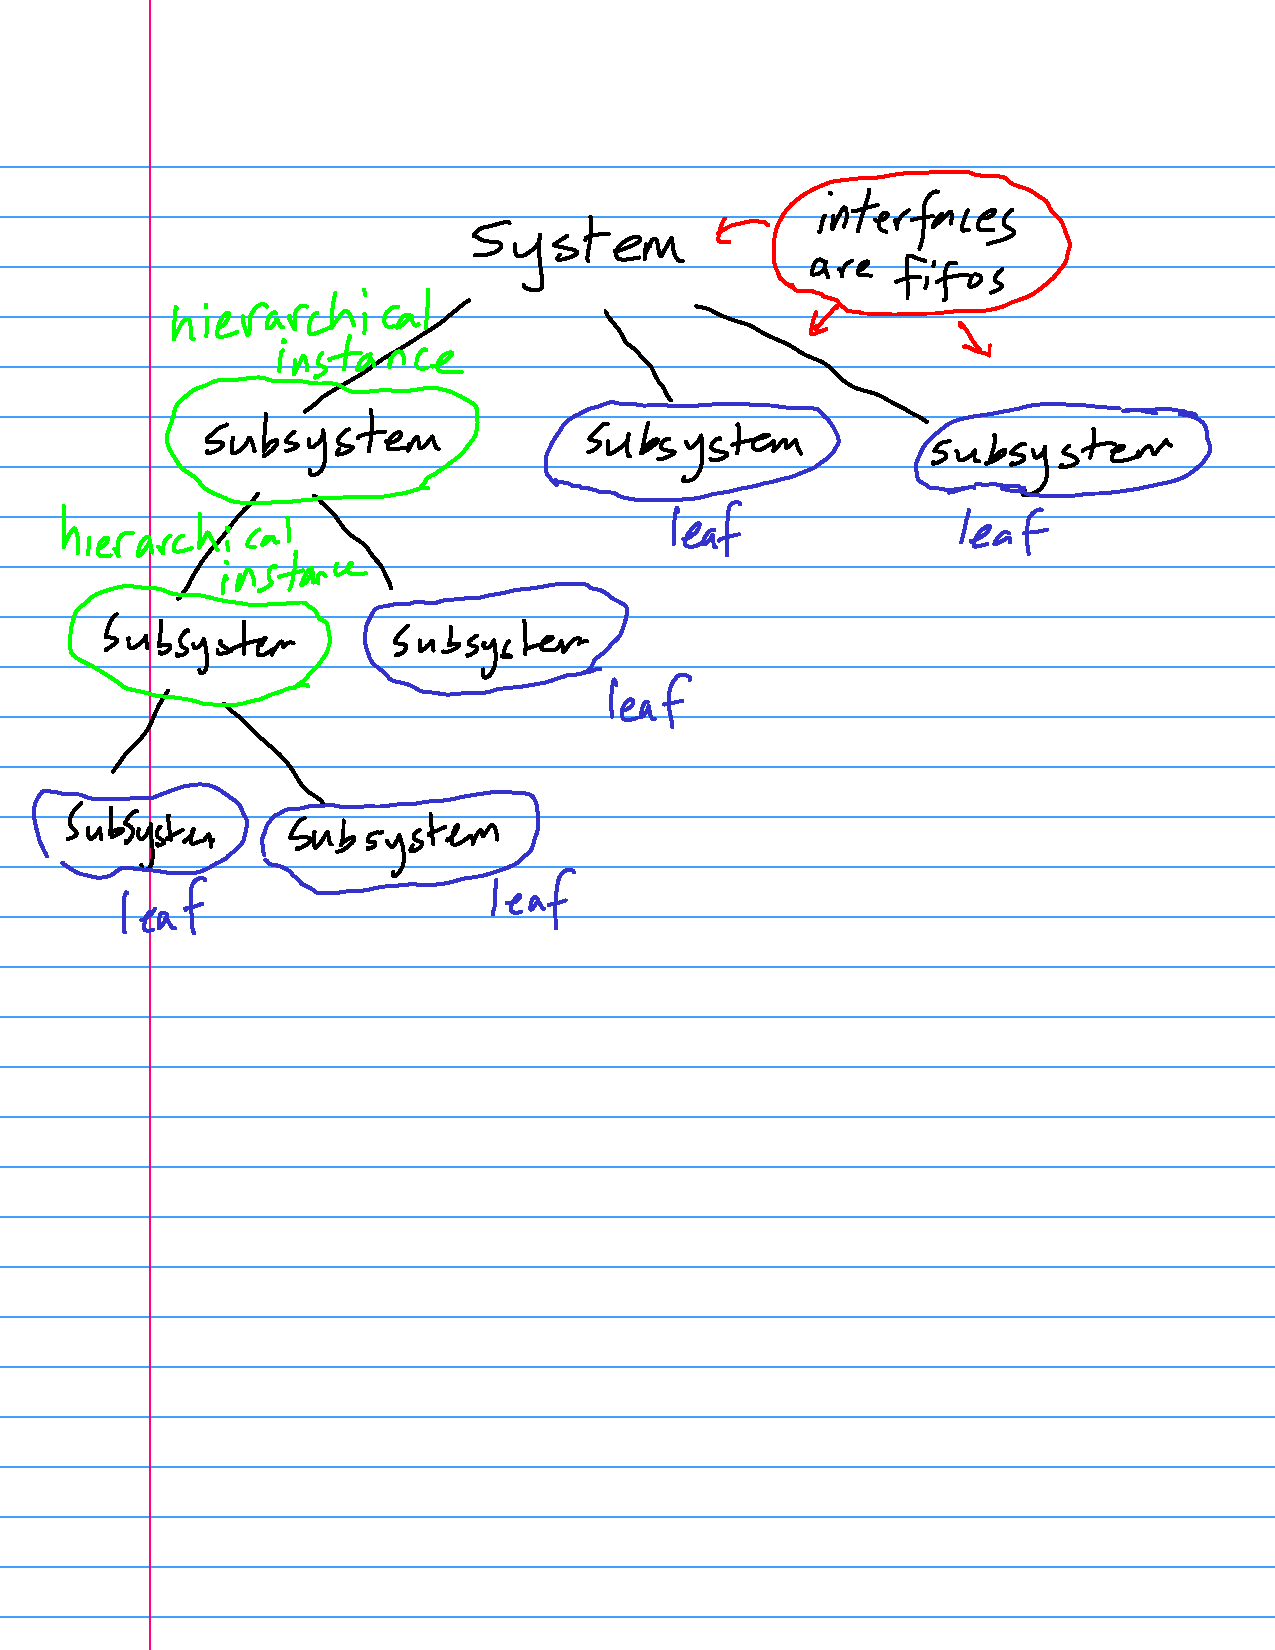
\includegraphics[width=10cm]{figs/hierarchy.pdf}
\caption{Visualization of the hierarchy}
\label{fig:hierarchy}
\end{figure}

The hierarchical description consists of a top-level system, which
can in turn instantiate sub-system instances, which are in turn constructed
using sub-systems.  There are two kinds of sub-system instances
\begin{itemize}
\item Hierarchical sub-system instances:  these are themselves constructed using
lower level instances.
\item Leaf sub-system instances: these are defined using {\bf C}, {\bf Aa} or
mixed {\bf C}/{\bf Aa} descriptions and consist of a collection of algorithmic
threads.
\end{itemize}

\subsection{Hierarchical sub-systems and their internal connections}

Hierachical sub-systems are purely structural and allow us to instantiate sub-systems
and connect them up.   Connections between sub-system instances can be of
two types
\begin{itemize}
\item FIFO connections:  Information from one sub-system instance can be sent to
another sub-system using FIFO buffers.  These buffers have two parameters, the
width (in bits) of the data that is written into and read from the FIFO, and the
depth of the FIFO, i.e., the number of elements it can store.
\begin{itemize}
\item Note that FIFOs are essentially blocking in nature, and serve as communication
and synchronization channels.
\end{itemize}
\item Signal connections: These are flags which can be used to exchange information
in a non-blocking (asynchronous) manner.
\end{itemize}

\subsection{Leaf sub-systems}

Leaf sub-systems are essentially a collection of threads which are described using
{\bf C} and {\bf Aa}.   These form the algorithmic heart of the overall system.


\subsection{Visualization of a typical system}

We show a visualization of a typical system in Figure \ref{fig:visualization}.
\begin{figure}
\centering
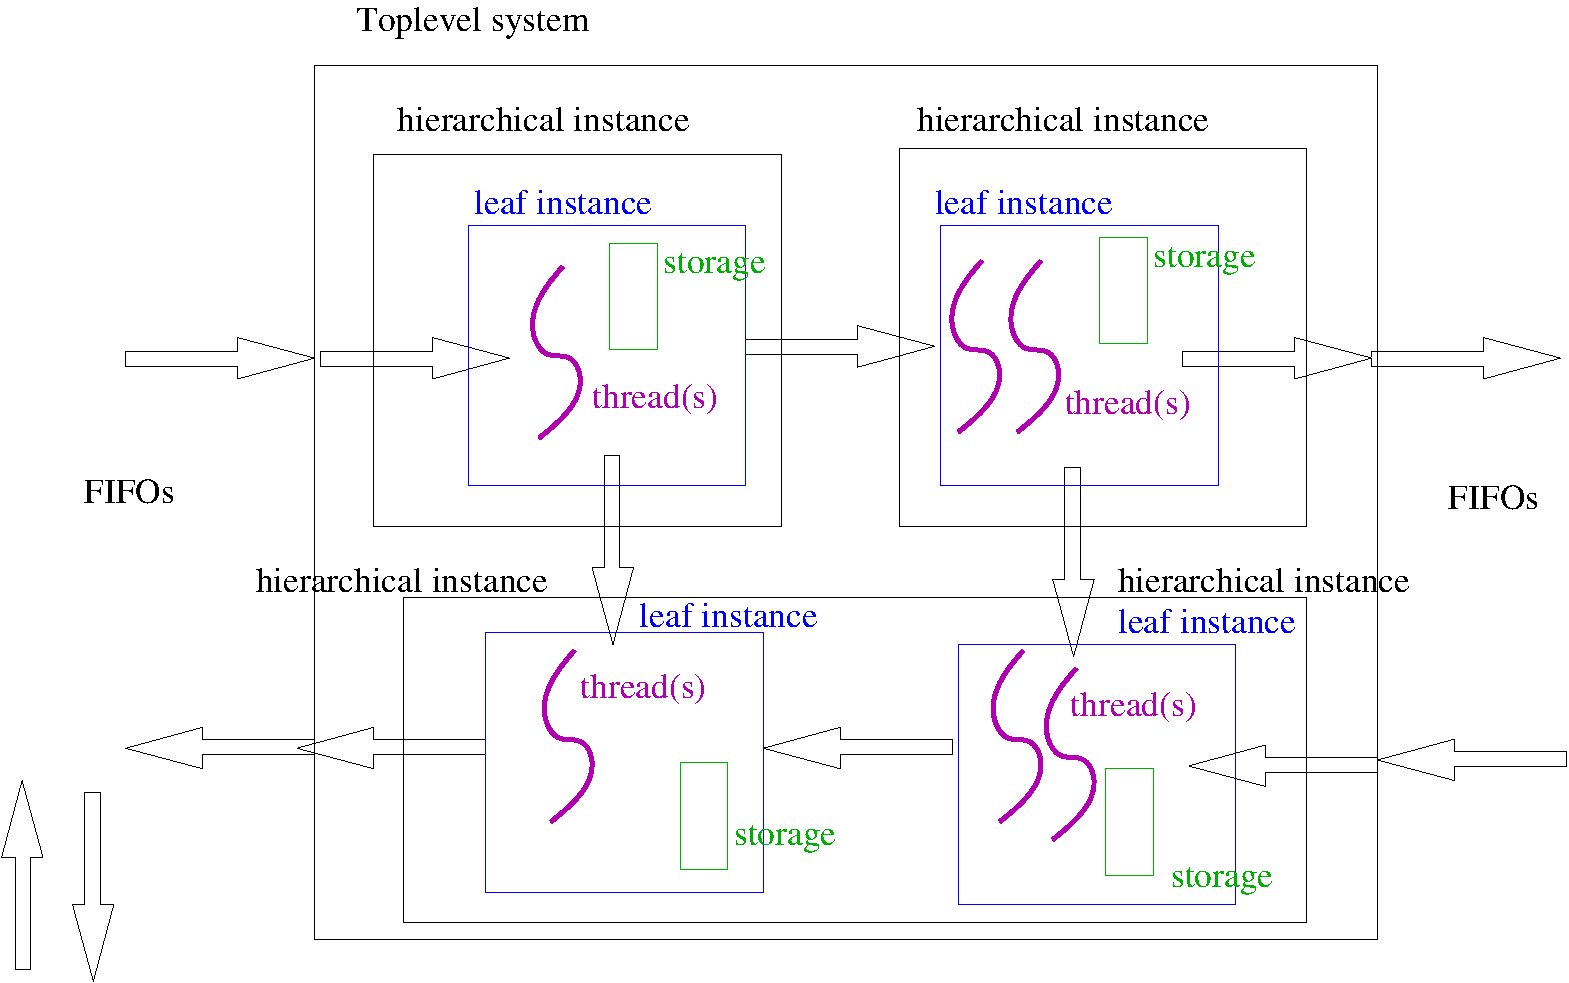
\includegraphics[width=10cm]{figs/visualization.pdf}
\caption{Visualization of a typical system}
\label{fig:visualization}
\end{figure}

The top-level system {\bf top} has three hierarchical sub-system instances {\bf top/i1}
{\bf top/i2} and {\bf top/i3}.  The hierachical sub-system instance {\bf top/i1} has
a single leaf-instance {\bf top/i1/i0}, etc.     The white arrows indicate FIFO
connections between sub-systems.

Each leaf instance will consist of a collection of threads, which can communicate
amongst them-selves using either the storage in the leaf instance or FIFOs.

\subsection{Summary}

The structure of a system is conventional but there are some important 
rules and restrictions.
\begin{itemize}
\item Hierarchical sub-system instances will interact only through FIFOs and signals.
\item A sub-system can be defined once and instantiated multiple times.
\item All storage will be declared and accessed from within leaf sub-system instances.
\end{itemize}

\section{Towards an AI/ML system description in the AHIR-V2 environment}

We start with a hierarchical description.  

\begin{verbatim}
$system ai_ml_engine $library ai_ml_lib
  $in
    $pipe INPUT_DATA
  $out
    $pipe OUTPUT_DATA
{
  $instance ictrl_inst 
      ai_ml_lib:input_controller

  $instance mem_inst
      ai_ml_lib:mem_pool 

  $instance processing_inst
      ai_ml_lib: processor_element 

  $instance octrl_inst
      ai-ml_lib: output_controller 
} 
\end{verbatim}

The system being describe here is the one shown in Figure \ref{fig:simpleExample}.
\begin{figure}
\centering
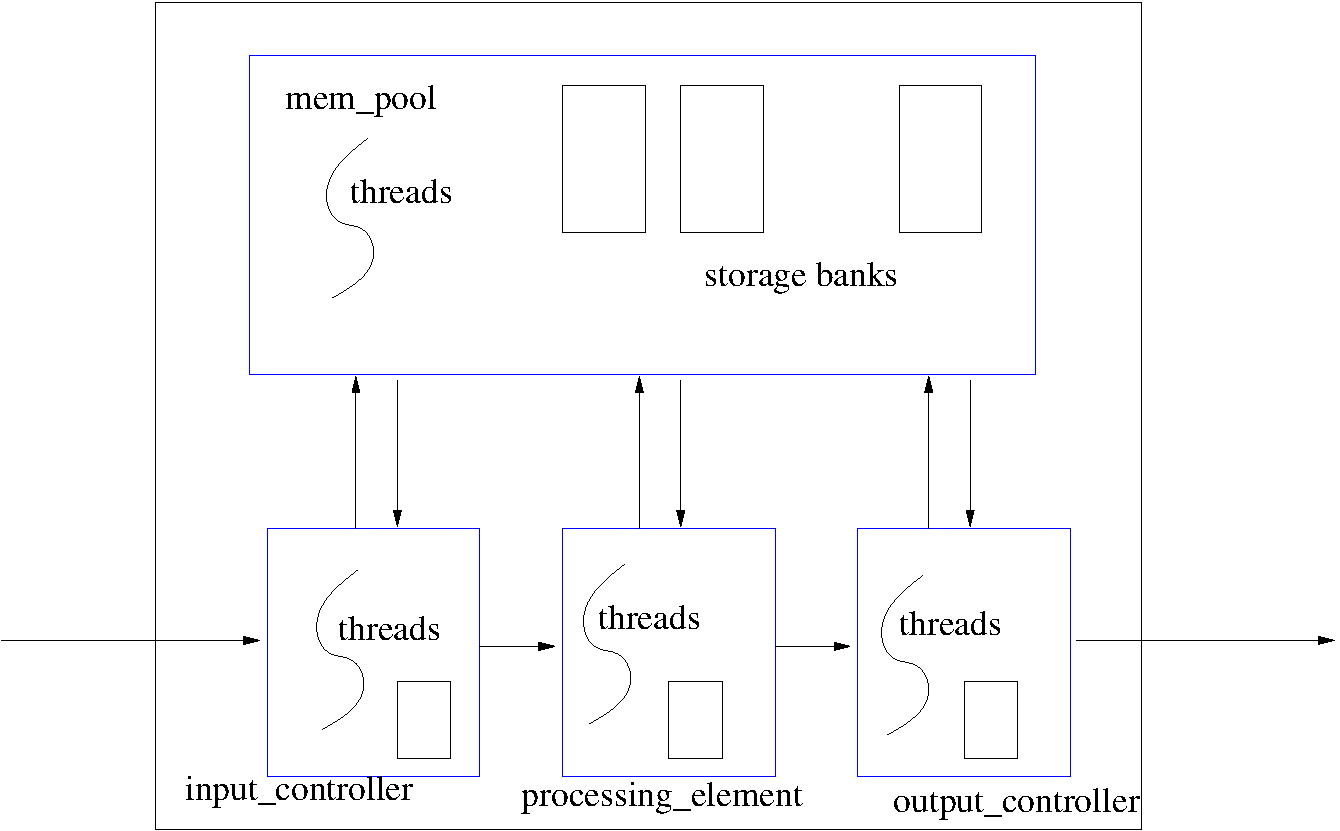
\includegraphics[width=10cm]{figs/simpleExample.pdf}
\caption{Simple AI/ML example}
\label{fig:simpleExample}
\end{figure}

The basic flow of information is as follows:
\begin{enumerate}
\item An input image is sent into the system using the FIFO from the left.
\item The input controller requests the memory pool to provide a memory
area to store the image.
\item The memory pool provides the storage area if available (as a buffer index).
\item The input controller stores the image into the memory pool, and
passes the buffer index to the processing element.
\item The processing element works on the image, using the memory pool and
its local storage for the processing.
\item Once done, the processing element passes an output data index to the
output controller.
\item The output controller picks up the output data from the memory pool
using this output data index and sends it out on the FIFO to the right.
\end{enumerate}

We will need to describe the threads that constitute the behaviour of
the four leaf sub-systems using either {\bf C} or {\bf Aa} or a combination
of the two.

\section{Towards a templatized AI/ML system description}

In this project, we will move a step above the description level described
in the previous section.
\begin{itemize}
\item We will define a set of leaf sub-system functions that are essential.
\item We will develop a parametrized model for a memory pool which can
be flexibly used in various configurations (size of memory, parallelism, number
of input ports, internal buffer classes).
\begin{itemize}
\item The physical implementation of these memories can be in FPGA block RAM
or in off FPGA DRAM.
\end{itemize}
\item We will define a simple language to show the structuring of the AI
system using the essential leaf sub-system functions, and memory pools.
\item From this description, we will generate a hierachical system description
as in the previous section.
\item Tools for mapping the hierarchical system description to VHDL 
are already available as part of the AHIR-V2 tool-set.
\end{itemize}

\subsection{First stage: understand the existing tools, and providing a reference implementation of the leaf functions}

Some introduction to the use of {\bf C} and {\bf Aa} for implementing 
hardware was covered in EE789.  However, I will provide a crash training
program for familiarization with the AHIR-V2 toolset in the hierarchical
system construction context.

We will simultaneously need to have reference implementations for the leaf functions.
The milestones are:
\begin{itemize}
\item Familiarity with AHIR-v2 tools:
\begin{itemize}
\item Demonstrated on FPGA for an image filter.
\end{itemize}
\item Reference C implementations of leaf functions.
\begin{itemize}
\item Demonstrated on hello\_world AI/ML application.
\end{itemize}
\end{itemize}

\subsection{Second stage: put together a pilot system using the existing AHIR-V2 tools}

This will require us to implement the leaf functions in {\bf C} and {\bf Aa} put them
together using the AHIR-V2 toolset and validate on FPGA.

We will simultaneously implement a memory pool which is backed by block RAM as well
as by DRAM.
The milestones are:
\begin{itemize}
\item Validated parametrizable memory pool backed by SRAM and DRAM.
\item Implementation of leaf functions in {\bf C}/{\bf Aa} demonstrated on
hardware.
\item Progress towards templatization language.
\end{itemize}

\subsection{Third stage: templatized construction of an AI/ML system}

A simple language and assembler to put together an entire system.


\end{document}
